
% drawio link: https://drive.google.com/open?id=10yQD3nL_LmK5xsChKugc4OlRGO5AMMoz
\begin{figure*}[!t]
    \centering
    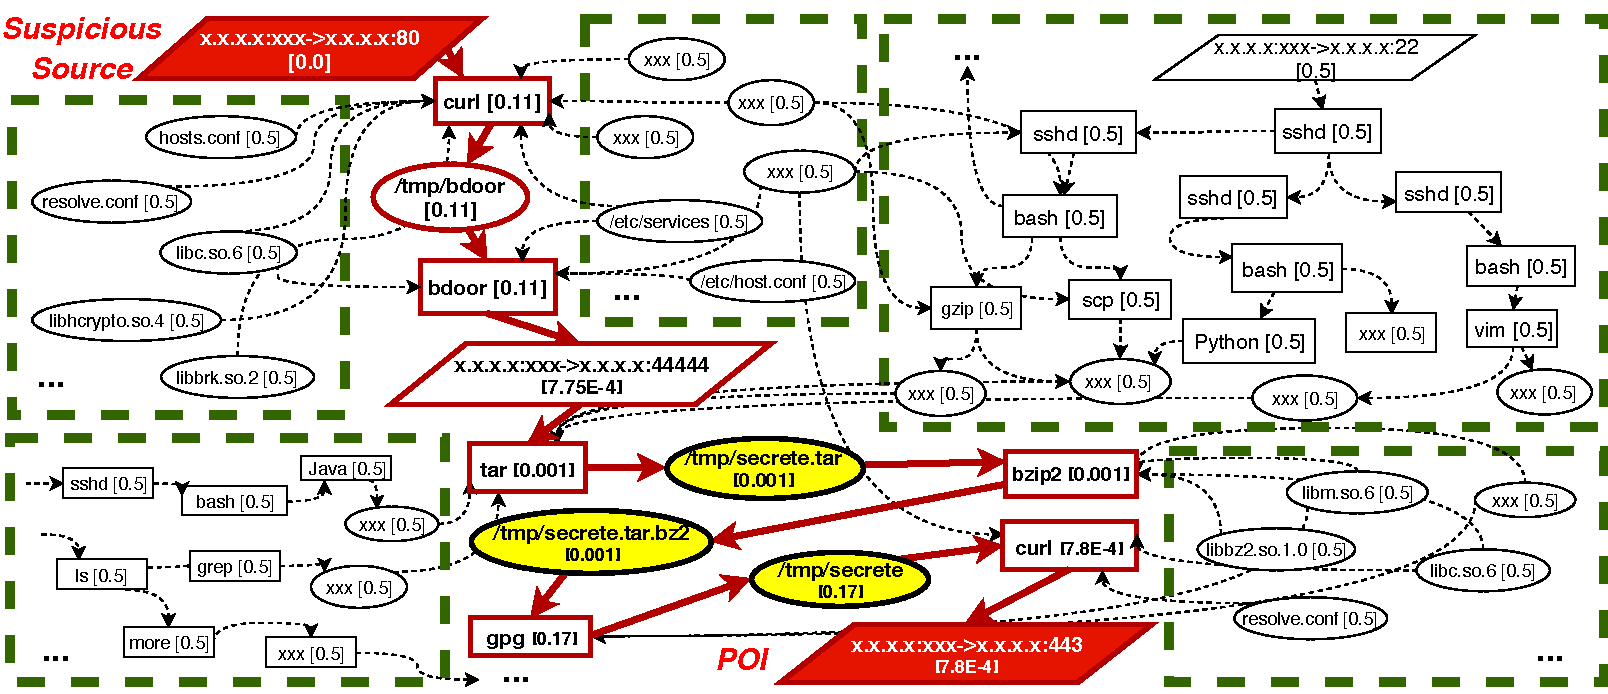
\includegraphics[width=0.98\textwidth]{figs/overview.pdf}
    \caption{Partial dependency graph of a motivating data leakage attack case. Rectangles denote processes, ovals denote files, and parallelograms denote network sockets. Yellow ovals are the files leaked in this attack. Nodes in the attack path have red frames while normal activities and system libraries are in dashed green rectangles. Critical edges are represented with solid red arrows. Non-critical edges are represented with dashed arrows. The complete graph contains 5,817 nodes and 215,380 edges. Note that the reputation of the suspicious source on the top left propagates mainly through the critical edges.}
   % \vspace{2mm}
    \label{fig:motivate}
\end{figure*}

\section{Background and Motivating Example}
\subsection{System Monitoring}
\label{subsec:system-monitoring}

System monitoring collects auditing events about system calls that are crucial in security analysis, describing the interactions among system entities.
%and resources.
As shown in previous studies~\cite{backtracking,backtracking2,taser,wormlog,gao2018saql,gao2018aiql,mcitracking,logtracking,liu2018priotracker,hassan2019nodoze}, on mainstream operating systems (Windows, Linux, and Mac OS), system entities in most cases are files, processes, and network connections,
and the collected system calls are mapped to three major types of system events:
(i) file access, 
(ii) processes creation and destruction, and
(iii) network access.
As such, we consider \emph{system entities} as \emph{files}, \emph{processes}, and \emph{network connections}.
We consider a \emph{system event} as the interaction between two system entities represented as \emph{$\langle$subject, operation, object$\rangle$}. Subjects are processes originating from software applications (\eg Chrome), and objects can be files, processes, and network connections. 
We categorize system events into three types according to the types of their object entities, namely \emph{file events}, \emph{process events}, and \emph{network events}.


Both entities and events have critical security-related
attributes (\cref{tab:entity-attributes,tab:event-attributes}).
The attributes of entities include the properties to support various security analyses
(\eg file name, process name, and IP address), and the
unique identifiers to distinguish entities (\eg file path, process name and PID, IP and port).
The attributes of events include event
origins (\eg start time/end time), operations (\eg file read/write), and other security-related properties (\eg failure code). 
%(\eg system call return code).

%%%%%%%%%%%%%%%%%%%%%%%%%%
\subsection{Causality Analysis}
\label{subsec:causality-analysis}

Causality analysis~\cite{backtracking,backtracking2,taser,intrusionrecovery,liu2018priotracker} analyzes the auditing events to infer the dependencies among system entities and present the dependencies as a directed graph.
%
In the dependency graph $G(E,V)$, a node $v \in V$ represents a process, a file, or a network network.
An edge $e(u, v) \in E$ indicates a system auditing event involving two entities $u$ and $v$ (\eg process creation, file read or write, and network access), and its direction (from the source node $u$ to the sink node $v$) indicates the data flow.
Each edge is associated with a time window, $tw(e)$.
We use $ts(e)$ and $te(e)$ to represent the starting time and the ending time of $e$.
Formally, in the dependency graph, for two event edges $e_1(u_1, v_1) $ and $e_2(u_2, v_2)$, there exists causal dependency between $e_1$ and $e_2$ if $v_1 = u_2$ and $ts(e_1) < te(e_2)$.

Causality analysis enables two important security applications:
(i) \emph{backward causality analysis} that helps identify the entry points of attacks, and (ii) \emph{forward causality analysis} that helps investigate the ramifications of attacks.
Given a POI event $e_s(u,v)$, a backward causality analysis traces back from the source node $u$ to find all events that have causal dependencies on $u$,
and a forward causality analysis traces forward from the sink node $v$ to find all events on which $v$ has causal dependencies.




\begin{table}[t]
	\centering
	\caption{Representative attributes of system entities}
	\label{tab:entity-attributes}
	\resizebox{0.44\textwidth}{!}{%
		\begin{tabular}{l|l|l}
			\hline
			\textbf{Entity}             & \textbf{Attributes}    & \textbf{Shape in Graph} \\ \hline
			File               & Name, Path          & Ellipse        \\
			Process            & PID, Name, User, Cmd  & Square         \\
			Network Connection & IP, Port, Protocol   & Parallelogram  \\ \hline
		\end{tabular}%
	}
\end{table}


% \eat{
% \begin{table}[!t]
% 	\centering
% 	\caption{Representative attributes of system entities}\label{tab:entity-attributes}
% 	\begin{adjustbox}{0.45\textwidth}
% 		\begin{tabular}{|l|l|}
% 			\hline
% 			\textbf{Entity}		&\textbf{Attributes}\\\hline
% 			File				&Path\\\hline
% 			Process			&PID, Name, User, Cmd\\\hline
% 			Network Connection	& IP, Port, Protocol \\\hline
% 		\end{tabular}
% 	\end{adjustbox}
% 	%	\vspace*{-2ex}

% 	\vspace*{1ex}
% \end{table}
% }
\begin{table}[!t]
	\centering
	\caption{Representative attributes of system events}
	\label{tab:event-attributes}
	\begin{adjustbox}{width=0.44\textwidth}
		\begin{tabular}{l|l}
			\hline
			\textbf{Operation}		& Read/Write, Execute, Start/End\\\hline
			\textbf{Time}		& Start Time/End Time, Duration\\\hline
			\textbf{Misc.}		& Subject ID, Object ID, Data Amount, Failure Code\\\hline
		\end{tabular}
	\end{adjustbox}
	%	\vspace*{-2ex}

	%	\vspace*{1ex}
\end{table}


\eat{
\begin{table}[!t]
	\centering
	\caption{Representative attributes of system events}\label{tab1:event-attributes}
	\begin{adjustbox}{width=0.48\textwidth}
		\begin{tabular}{|l|l|}
			\hline
			Operation		& Read/Write, Execute, Start/End, Rename/Delete.\\\hline
			Time/Sequence		& Start Time/End Time, Event Sequence\\\hline
			Misc.		& Subject ID, Object ID, Failure Code\\\hline
		\end{tabular}
	\end{adjustbox}
	%	\vspace*{-2ex}

		\vspace*{1ex}
\end{table}
}


%%%%%%%%%%%%%%%%%%%%%%%%
\subsection{Motivating Example}
\label{subsec:motivating-example}

\cref{fig:motivate} shows an example dependency graph of a data leakage attack:
the attacker exploited the shellshock bug to execute \incode{curl} in the target system and downloaded a backdoor program \incode{bdoor}. The attacker then executed the \incode{bdoor} program to open a backdoor
%port 
on port 44444. Through the backdoor, the attacker collected sensitive data using \incode{tar}, \incode{bzip2}, and \incode{gpg}, and uploaded the collected data to a remote host.
The POI entity is a network connection to the suspicious remote host. The complete graph contains 5,817 nodes and 215,380 edges, which is impractical for a human analyst to manually inspect.
%which is a non-trivial task for human analyzer. 

\tool enables automatic attack investigation by assigning weights to edges and propagating reputation scores from seed sources to POI entities.
In this example, we set the reputation score for the suspicious network source (\ie the top left parallelogram)
%that initiates the attack as 
to $0.0$ and the reputation scores for 
%other 
system libraries to $0.5$.

\myparatight{Challenges} 
From \cref{fig:motivate}, we can see that the critical edges (\ie the red bold edges) representing the attack sequence are buried in many irrelevant system activities, such as remote login via ssh and normal program execution like Java and Python.
Thus, \tool needs to assign high weights to the critical edges to distinguish them from edges representing irrelevant system activities, 
and propagates reputation scores based on the weights to ensure that the critical edges have the most impact on the POI entity. 
Furthermore, the dependency path from the suspicious source to the POI entity has more than 10 hops, where each node in the middle of the path also receives reputation from other sources.
As such, \tool needs to make sure that the reputation propagation does not suffer from fast degradation in a long path with many irrelevant nodes that can potentially distort the final reputation score.

\myparatight{Techniques of \tool} 
\tool first computes the weights using three novel discriminative features (\cref{subsec:feature-extraction}).
In this example, compared with other (\ie non-critical) edges, the critical edges have more similar data amount as the data amount transmitted in the POI event, the start timestamps of these edges are closer to the POI event, and the incoming and outgoing edges are relatively small for the nodes involved in the critical edges.
Thus, by combining these features into the edge weights (\cref{subsec:weight-computation}), \tool maximizes the differences between critical edges and other edges, and reveals the critical edges.
Based on the weights, \tool adopts an inheritance fashion that considers the impact of the edges to propagate the reputation scores from the seed sources in the graph (\cref{subsec:attack-investigation}).
%
From \cref{fig:motivate}, we observe that the reputation scores of nodes on the critical edges are close to $0$, as compared to the irrelevant system libraries with reputation scores close to $0.5$.
By connecting the nodes with low reputation scores and the critical edges, we are able to reconstruct the attack sequence.
We also observe that the POI entity receives a very low reputation score that is almost $0$, which indicates that it comes from a suspicious source as expected.

      

% process \incode{script.py} executes \incode{wget} to download a file named \incode{wget-1.19.zip}, and unzips it to obtain the file \incode{INSTALL}.
% Such task is often seen in malicious payloads~\cite{securitybook}.
% The POI event of the graph is the event that creates the file \incode{INSTALL}.
% The original dependency graph obtained by applying causality analysis on the POI event contains 86 nodes and 7211 edges.
% Due to space limit, only relevant part is shown in the figure.

% \begin{figure}
%     \centering
%     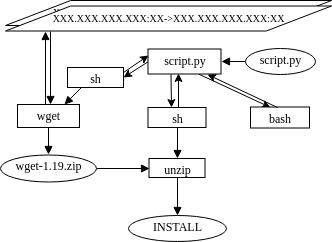
\includegraphics[width=0.4\textwidth]{figs/after.png}
%     \caption{The critical edges of the dependency graph in Fig.~\ref{fig:before}}
%     \label{fig:after}
% \end{figure}

\eat{

By assigning weights to the edges and propagate reputation from the seed (in this case, the seed is the network socket at the most top left.), our system enables analysts to reconstruct the attack path in a reasonable time. 

\myparatight{Revealing Critical Edges}
The first goal of attack investigation using dependency graph is to surface attack provenance, \ie finding critical edges.
\cref{fig:after} shows the 14 critical edges of the example dependency graph.
Obviously, it requires non-trivial efforts to search these critical edges from the huge dependency graph with 86 nodes and 7211 edges, and there is a strong need to automate this identification process.

However, causality analysis~\cite{backtracking,backtracking2} typically uses time windows to make decisions on whether an edge has causal dependency on the POI event, which contains limited information to distinguish critical edges.
For example, the \incode{script.py} process node has many incoming edges, but the edges marked in blue are coming from system libraries, which give little information on surfacing the attack provenance, while the edges that connect to the process \incode{sh} show much more useful information for investigating the task.
But all these edges cannot be pruned since the end times of their time windows are all before the POI event. 

To address this challenge, \tool leverages the insight that critical edges often possess properties that are different from non-critical edges: (i) the time difference between the critical edges and the POI event is usually small;
(ii) the data amount processed by the critical edges is similar to the target file in the POI event;
(iii) source nodes of non-critical edges have either no incoming edges (\eg system libraries) or many outgoing edges (\eg long-running processes), while the source node of the critical edges usually has only a few incoming edges and only a few outgoing edges (\ie ``high concentration'').
To capture these properties, \tool computes three novel features for each edge: \emph{relative time difference}, \emph{relative data amount difference}, and \emph{concentration degree} (details in \cref{sec:approach}), and use them to determine the weight for each edge, producing a weighted dependency graph.

Note that with the weights on the edges, security analysts can control the threshold value on hiding some non-critical edges with low weights when identifying the critical edges.
But when the security analysts need to look into some part of the graph with more details,
he may lower the threshold value and the non-critical edges that contain more detailed information (\eg library files) will be shown.

\myparatight{Reputation Propagation}
The second goal of attack investigation using dependency graph is to determine whether the file \incode{INSTALL} contains malicious payloads. 
If we look at the critical edges, we can trace back from \incode{INSTALL} to \incode{script.py}, which is the creator of \incode{INSTALL}.
This indicates that if \incode{script.py} is suspicious, \incode{INSTALL} is very likely to contain malicious payloads; otherwise, \incode{INSTALL} is likely to be a benign installation script.

To automate the process in inspecting the dependency graph for determining whether a POI event contains malicious payloads, \tool performs reputation propagation on the weighted dependency graph.
In this example, if we assume \incode{script.py} is suspicious (\ie $0$), and all the system libraries with a neural reputation (\ie 0.5).
Then \tool propagates the reputation from these seed nodes through all the edges, where the weights of the edges are proportional to the reputation being propagated from the nodes.
Thus, if the weights of the critical edges are significantly higher than the weights of the non-critical edges, the contribution from \incode{script.py} to \incode{wget} dominates the contributions from system libraries to \incode{wget}.
This will cause \incode{INSTALL} to have a reputation close to 0, which is similar to \incode{script.py}, but not the system libraries.
In this way, \tool can automatically determine that \incode{INSTALL} is very likely to contain malicious payloads.
}